\section{Experiments}\label{sec:experiments}

\subsection{Datasets}

The performance of our collaborative preference model with the BALD active learning strategy
is evaluated in a series of experiments with simulated and real-world data. The datasets were 
pre-processed as follows.

{\bf Synthetic.} We generated $10$ items with feature vectors $\mathbf{x}_i=(x_{i1},x_{i2})$,
where $x_{i1}$ and $x_{i2}$ are uniformly distributed with zero mean and unit variance, for $i = 1,\ldots,10$.
The user preferences are obtained
using $D=5$ latent functions $h_1,\ldots,h_5$ sampled from a Gaussian process
with zero mean and preference kernel given by a squared exponential kernel with unit length-scale.
The preferences for the $u$-th user are generated according to the sign of
$g_u(\mathbf{x}_i, \mathbf{x}_j) = \sum_{d=1}^5 w_{d}'(\mathbf{u}_u) h_d(\mathbf{x}_i, \mathbf{x}_j) + \epsilon_{ij}$,
where $\epsilon_{ij} \sim \mathcal{N}(0,1)$, the user features $\mathbf{u}_u$ are
generated in the same manner as the feature vectors for the items and the functions $w_{1}',\ldots,w_{D}$
follow the same prior distribution as $h_1,\ldots,h_5'$.

{\bf Jura.} 
This dataset contains concentration measurements for 7 heavy metals in soils of the Swiss Jura region at 359 locations \citep{Atteia1994315,Webster1994}.
We standardized the measurements of each heavy metal to have zero mean and unit standard deviation across the whole dataset.
The standardized measurements are used as utility values to generate preferences for any pair of heavy
metals at each location. Therefore, in this dataset, the locations correspond to users and each heavy metal
represents a different item. To generate the item features, we randomly singled out 20 locations.
The item features are given by the standardized measurements obtained at these locations. 
The user features correspond to the $x$ and $y$ coordinates for the measurements as well as the rock and land type.

{\bf MovieLens.} 
This dataset contains 1 million ratings from 6,000 users on 4,000 movies.
A total of 10 movies were randomly selected from the 50 movies with most ratings.
We also selected those users with at least 7 ratings on these 10 movies.
The remaining missing ratings were estimated using a nearest neighbor method.
The ratings for each user were used as utility values in order to generate preferences for each pair of movies.
The features for each user are gender, age and occupation. The features for each movie are genres
such as \emph{action}, \emph{comedy} or \emph{adventure}.

{\bf Sushi.}
This dataset contains complete rankings given by 5,000 users on $10$ different types of sushi \citep{Kamishima05},
where each sushi includes as features style, major group, minor group, heaviness, consumption
frequency, normalized price and sale frequency. The different users are also represented by
a set of features which include gender, age and geographical/regional information.

{\bf Election.}
This dataset contains the votes obtained by 8 political parties (items) at 650 constituencies (users) in
the 2010 general elections in the UK.
We only kept data for those constituencies with at least votes for more than 6 parties. Missing votes
were estimated using a nearest neighbor method. To generate feature vectors for each item,
we randomly singled out 20 constituencies and used the corresponding votes as features.
The features for each `user' are the corresponding coordinates (latitude and longitude) of the centroid of the constituency on the map.


\subsection{Tuning the kernel lengthscale}

\begin{figure}
\centering
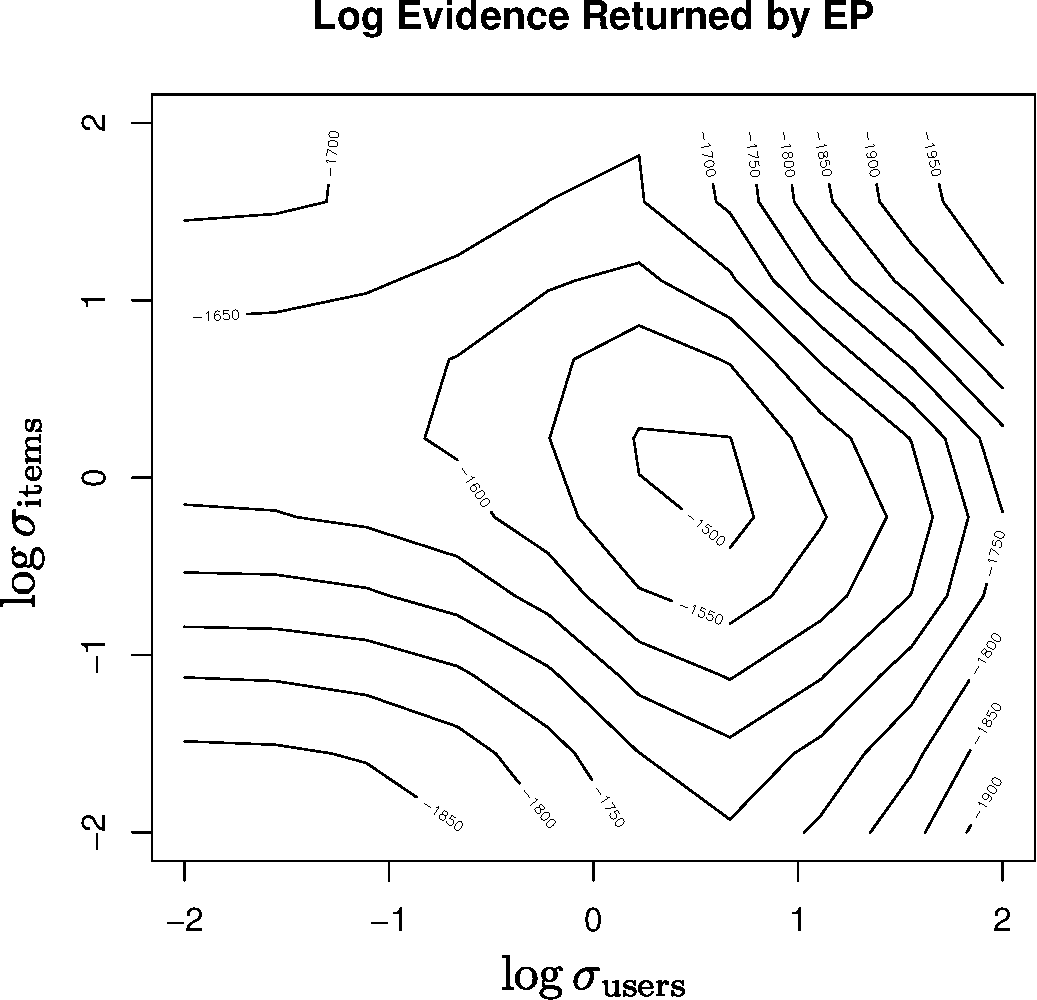
\includegraphics[scale=0.4]{figs/plotEvidence.pdf}
\caption{Logarithm of the evidence returned by EP when run on the first training set of the experiments with synthetic data.
Different values are considered for the lengthscale parameters $\sigma_\text{users}$ and $\sigma_\text{items}$.
The synthetic data are generated using $\log \sigma_\text{users} = 0$ and $\log \sigma_\text{items} = 0$.
The highest evidence returned by EP corresponds to values of $\log \sigma_\text{users}$ and
$\log \sigma_\text{items}$ close to zero.}\label{fig:experimentEvidence}
\end{figure}

Before the main experiments we perform an initial investigation to show that approximation of the model evidence given by EP can be used to
tune the kernel hyper-parameters in the proposed multi-user model. For this, we use the synthetic dataset
described in the main document. Figure \ref{fig:experimentEvidence} shows a contour plot of the log-evidence returned by EP 
when run on the first training set of the experiments with synthetic data and 100 users.
Different values are considered for the lengthscale parameters $\sigma_\text{users}$ and $\sigma_\text{items}$.
The synthetic data are generated using $\log \sigma_\text{users} = 0$ and $\log \sigma_\text{items} = 0$.
The highest evidence returned by EP corresponds to values of $\log \sigma_\text{users}$ and $\log \sigma_\text{items}$ close to zero.
In this experiment we are running EP using a total of 20 latent functions,
while the data are generated using only 5 latent functions.
As mentioned in the main document, the proposed multi-user model
seems to be robust to over-fitting and over-estimation of
the number of latent functions does not seem to harm predictive performance.

\subsection{Comparison with other multi-user methods}

\paragraph{Alternative models.} Two versions of the proposed collaborative preference (CP) model are used.
The first version (CPU) takes into account the available user features, as described in Section \ref{sec:model}. The second version (CP) ignores these features by
replacing $\mathbf{K}_\text{users}$ in (\ref{eq:priorW}) with the identity matrix.
We compare to the two multi-user methods described in Section \ref{sec:relatedWork}. 
We denote to the model of Birlutiu \emph{et al.} as (BI), and that of
Bonilla \emph{et al.} as (BO).
We implement BO and BI using the preference kernel and EP for approximate inference.
Remember, that BI does not incorporate user features, and BO must include them.
Finally, we consider a single user approach (SU) which fits a different GP classifier independently to the data of each user.

\paragraph{Experimental procedure.} Due to the high computational cost of BI and BO, to compare to these methods we must subsample the datasets, keeping only 100 users.
The available data were split randomly into training and test sets of item pairs,
where the training sets contain 20 pairs per user in Sushi, MovieLens and Election, 15 pairs in Jura and
30 in Synthetic. This was repeated 25 times to obtain statistically meaningful results.
In CPU and CP, we selected the number of latent functions $D$ to be $20$ (see Table \ref{tab:small}).
In general, the proposed models, CPU and CP, are robust to over-fitting and over-estimation of
$D$ does not harm predictive performance. Note that the Synthetic dataset is generated
using $D=5$ and CPU and CP still obtain very good results using $D = 20$.
This automatic pruning of unnecessary degrees of freedom seems to be common
in methods based on variational Bayes \cite{MacKay2001}.
We selected the kernel lengthscales to be equal to
the median distance between feature vectors. This leads to good empirical performance
for most methods. An exception is BO, where the kernel hyperparameters
are tuned to some held-out data using automatic relevance determination.
In our model, we can also estimate the kernel
lengthscales by maximizing the EP approximation of the model evidence,
as illustrated in the Supplementary material. This alternative approach can be used
when it is necessary to fine tune the lengthscale parameters to the data. In CPU we use $U_0 = 25$ pseudo inputs for approximating $\mathbf{K}_\text{users}$.
These pseudo inputs are selected randomly from the set of available data points.
Similarly, in CP and CPU, we use $P_0 = 25$ pseudo inputs for approximating $\mathbf{K}_\text{items}$,
except in the Jura and Election datasets (which contain fewer items) where we use $P_0 = 15$.
The results obtained are not sensitive to the number of pseudo inputs used, as long as
the number is not excessively low.

%\renewcommand{\arraystretch}{0.9}
\newcommand{\ic}{\hspace{0.25cm}}
\begin{table}
\begin{minipage}[b]{0.49\columnwidth}
\centering
\caption{Average test error with 100 users.}
\resizebox{0.9 \columnwidth}{!}{
\begin{tabular}{@{\ic}l@{\ic}c@{\ic}c@{\ic}c@{\ic}c@{\ic}c@{\ic}c@{\ic}}
\hline
\textbf{Dataset} &\textbf{CPU}&\textbf{CP}&\textbf{BI}&\textbf{BO}&\textbf{SU}\\
\hline
Synthetic&0.162&0.180&0.175&\bf{0.157}&0.226\\
Sushi&0.171&0.163&\bf{0.160}&0.266&0.187\\
MovieLens&0.182&\bf{0.166}&0.168&0.302&0.217\\
Election&0.199&0.123&\bf{0.077}&0.401&0.300\\
Jura&0.159&\bf{0.153}&\bf{0.153}&0.254&0.181\\
\hline
\end{tabular} \label{tab:errorSmallDatasets}
}
\end{minipage}
\begin{minipage}[b]{0.5\columnwidth}
\centering
\caption{Training times (s) with 100 users.}
\resizebox{0.9 \columnwidth}{!}{
\begin{tabular}{@{\ic}l@{\ic}r@{\ic}r@{\ic}r@{\ic}r@{\ic}r@{\ic}r@{\ic}}
\hline
\textbf{Dataset} &\textbf{CPU}&\textbf{CP}&\textbf{BI}&\textbf{BO}&\textbf{SU}\\
\hline
Synthetic&7.793&9.498&22.524&311.574&0.927\\
Sushi&5.694&4.307&20.028&215.136&0.817\\
MovieLens&5.313&4.013&19.366&69.048&0.604\\
Election&13.134&12.408&20.880&120.011&0.888\\
Jura&3.762&2.404&15.234&88.502&0.628\\
\hline
\end{tabular} \label{tab:timeSmallDatasets}
}
\end{minipage}
\label{tab:small}
\end{table}



\paragraph{Results.} Average test errors are shown in Table \ref{tab:errorSmallDatasets}. 
Those highlighted in bold are statistically different to those not highlighted
(calculated using a paired $t$ test). Overall, CP and CPU outperform SU and BO, and breaks even with BI;
the final result is notable as BI learns the full mean and covariance structure across all users,
ours uses only a few latent dimensions, which provides the key to scaling to many more users.
CP outperforms CPU in all cases except in the Synthetic dataset. In the real-world datasets, users with 
similar features do not seem to have similar preferences and so correlating behavior of users with similar features is detrimental.
In this case, the unsupervised learning of similarities in user preferences is more useful for prediction than the user features.
This also explains the poor overall results obtained by BO.
Finally, running times in seconds are presented in Table \ref{tab:timeSmallDatasets}. 
The entries for BO do not include the time spent by this method to tune the kernel hyper-parameters.
CP and CPU are faster than BO and BI. The FITC approximation imposes
a large multiplicative constant in the cost of CP and CPU so for larger datasets the gains are much larger.

\subsection{Active learning on large datasets}

\renewcommand{\ic}{\hspace{0.3cm}}
\begin{table}
\centering
\caption{Test error for each method and active learning strategy with at most 1000 users. Standard deviations ommitted for readability.}
\resizebox{0.95\textwidth}{!}{
\begin{tabular}{@{\ic}l@{\ic}@{\ic}c@{\ic}c@{\ic}c@{\ic}@{\ic}c@{\ic}c@{\ic}c@{\ic}@{\ic}c@{\ic}c@{\ic}c@{\ic}}
\hline
\textbf{Dataset}&\textbf{CPU-B}&\textbf{CPU-E}&\textbf{CPU-R}&
\textbf{CP-B}&\textbf{CP-E}&\textbf{CP-R}&\textbf{SU-B}&\textbf{SU-E}&\textbf{SU-R}\\\hline
Synthetic&\underline{\bf{0.136}}&\bf\underline{{0.136}}&0.14&\bf{0.154}&0.161&0.179&\bf{0.253}&0.263&0.276\\
Sushi&\bf{0.150}&0.155&0.185&\underline{\bf{0.143}}&0.151&0.179&\bf{0.183}&0.199&0.215\\
MovieLens&\bf{0.172}&0.177&0.200&\underline{\bf{0.165}}&0.171&0.196&\bf{0.233}&0.24&0.253\\
Election&0.221&\bf{0.188}&0.265&\underline{\bf{0.107}}&\underline{\bf{0.103}}&0.184&\bf{0.331}&0.349&0.344\\
Jura&\bf{0.143}&\bf{0.144}&0.17&\underline{\bf{0.138}}&\underline{\bf{0.138}}&0.17&0.183&\bf{0.169}&0.201\\
\hline
\end{tabular}
}
\label{tab:large}
\end{table}


\begin{figure}[h!]
\centering
\resizebox{\textwidth}{!}{
\begin{tabular}{ccc}
Synthetic&
Sushi&
MovieLens\\
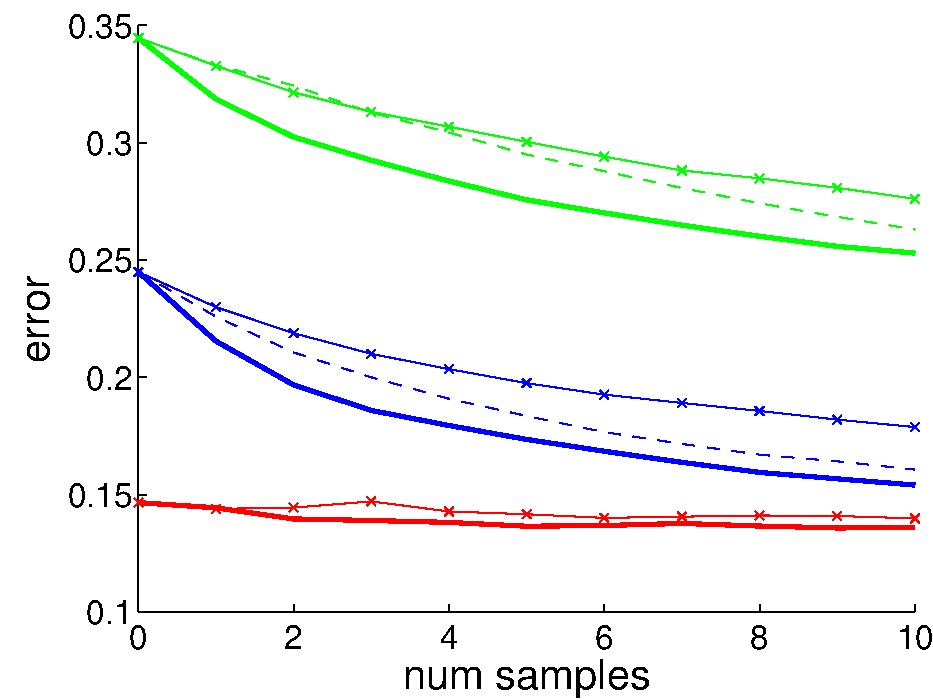
\includegraphics[scale=0.3]{figs/error_syntheticDataLargeScale.pdf}&
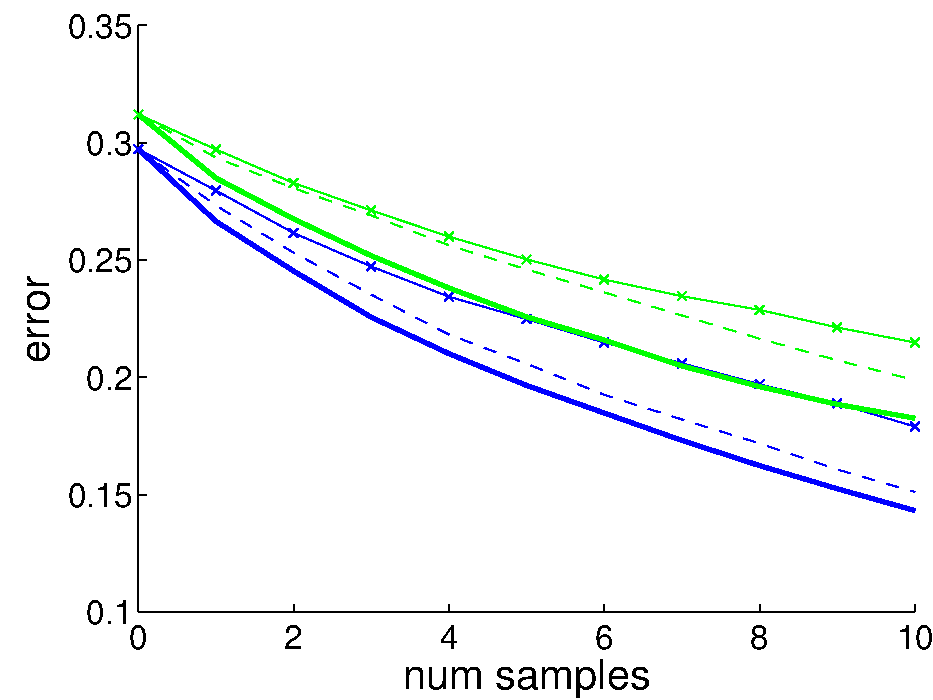
\includegraphics[scale=0.3]{figs/error_sushiDataLargeScale.pdf}&
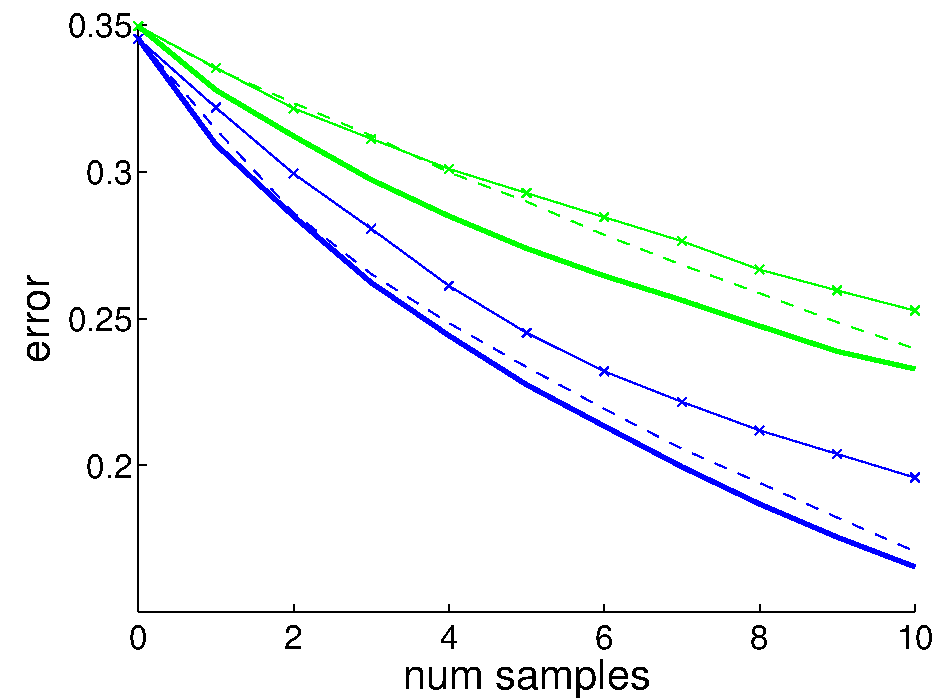
\includegraphics[scale=0.3]{figs/error_movieLensDataLargeScale.pdf}\\
Election&
Jura&
\\
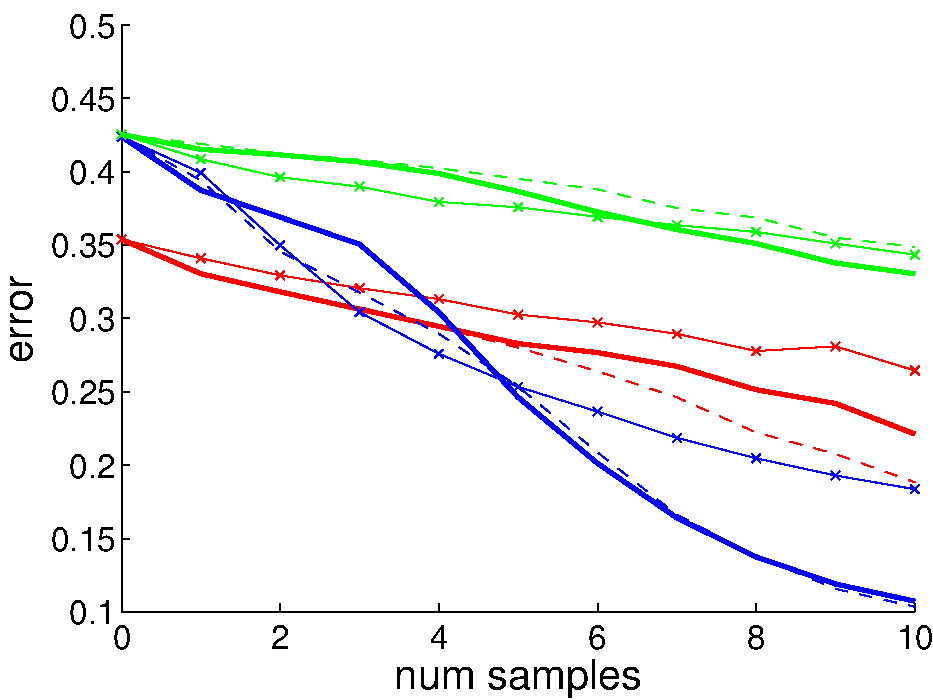
\includegraphics[scale=0.3]{figs/error_electionDataLargeScale.pdf}&
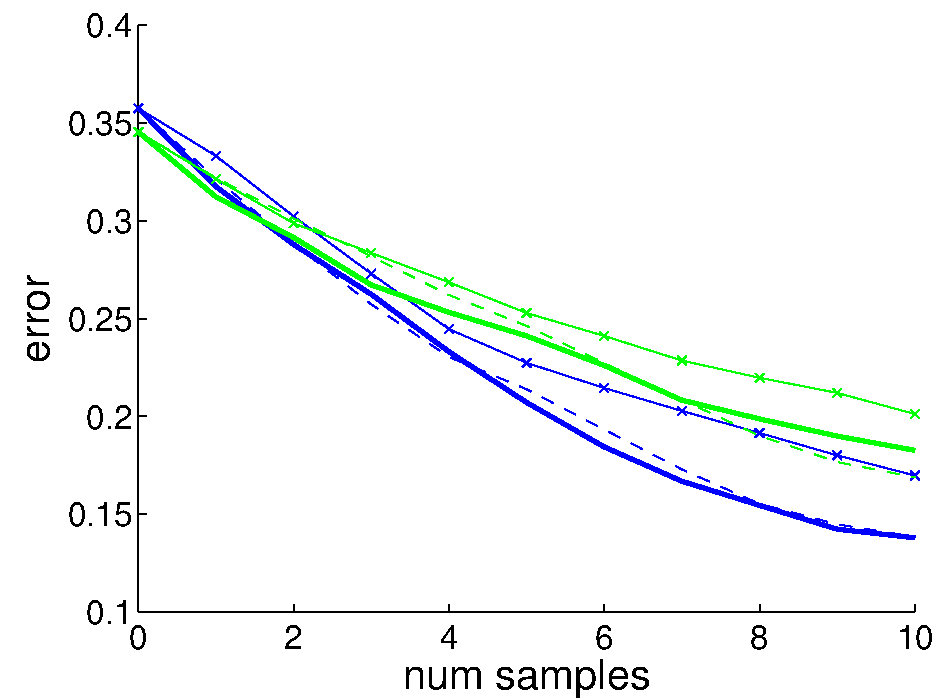
\includegraphics[scale=0.3]{figs/error_juraDataLargeScale.pdf}&
\hskip0.6cm \raisebox{0.08\height}{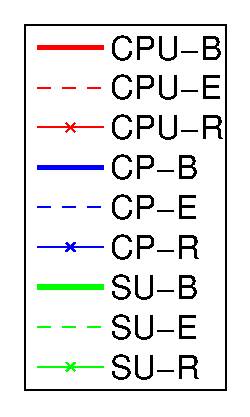
\includegraphics[scale=0.45]{figs/legend.pdf}}
\end{tabular}
}
\caption{Average test error for CPU, CP and SU, using the strategies BALD (-B), entropy (-E) and random (-R) for active learning.
For visual clarity, the curves for CPU are included only in the Synthetic and Election datasets.}
\label{fig:learningcurves}
\end{figure}

Here we evaluate the performance of BALD,
in particular, we compare CPU, CP, and SU using BALD (-B), Maximum Entropy Sampling (-E) and random sampling (-R).
We now use all the available users from each dataset, with a maximum of 1000 users.
For each user the available preference data are
split randomly into training, pool and test sets with 5, 35 and 5 data points respectively
in Synthetic, Sushi and MovieLens, 3, 22 and 3 data points in Election
and 3, 15 and 3 data points in Jura.
Each method is fitted using the training sets and its performance
is then evaluated on the corresponding test sets. After this,
the most informative data point is identified in each
of the pool sets. These data points are moved into the corresponding training sets
and the process repeats until 10 of these active
additions to the training sets have been completed.
The entire process, including the dataset splitting is repeated 25 times. 
Figure \ref{fig:learningcurves} shows the learning curve for each method.
For clarity, the curve for CPU is included only for the Synthetic and Election datasets; in the other datasets CPU is marginally outperformed by CP.
Average errors after 10 queries from the pool set of each user are summarized in Table \ref{tab:large}.
For each model (CPU, CP and SU), the results of the best active learning strategy are highlighted in bold.
The results of the best model/active learning strategy combination are underlined.
Highlighted results are statistically significant with respect to non-highlighted
results according to a paired $t$ test.
BALD always outperforms random sampling and usually outperforms or obtains equivalent performance to MES. 
In particular, BALD significantly outperforms MES in nine cases,
while MES is better than BALD in only two cases.
